%; whizzy chapter
% -initex iniptex -latex platex -format platex -bibtex jbibtex -fmt fmt
% 以上 whizzytex を使用する場合の設定。

%     Kansai Debian Meeting resources
%     Copyright (C) 2007 Takaya Yamashita
%     Thank you for Tokyo Debian Meeting resources

%     This program is free software; you can redistribute it and/or modify
%     it under the terms of the GNU General Public License as published by
%     the Free Software Foundation; either version 2 of the License, or
%     (at your option) any later version.

%     This program is distributed in the hope that it will be useful,
%     but WITHOUT ANY WARRANTY; without even the implied warranty of
%     MERCHANTABILITY or FITNESS FOR A PARTICULAR PURPOSE.  See the
%     GNU General Public License for more details.

%     You should have received a copy of the GNU General Public License
%     along with this program; if not, write to the Free Software
%     Foundation, Inc., 51 Franklin St, Fifth Floor, Boston, MA  02110-1301 USA

%  preview (shell-command (concat "evince " (replace-regexp-in-string "tex$" "pdf"(buffer-file-name)) "&"))
% 画像ファイルを処理するためにはebbを利用してboundingboxを作成。
%(shell-command "cd image200708; ebb *.png")

%%ここからヘッダ開始。

\documentclass[mingoth,a4paper]{jsarticle}
\usepackage{kansaimonthlyreport}
\usepackage{ascmac}

% 日付を定義する、毎月変わります。
\newcommand{\debmtgyear}{2008}
\newcommand{\debmtgdate}{23}
\newcommand{\debmtgmonth}{3}
\newcommand{\debmtgnumber}{11}

\begin{document}

\begin{titlepage}

% 毎月変更する部分, 本文の末尾も修正することをわすれずに

 第\debmtgnumber{}回 関西 Debian 勉強会資料

\vspace{2cm}

\begin{center}
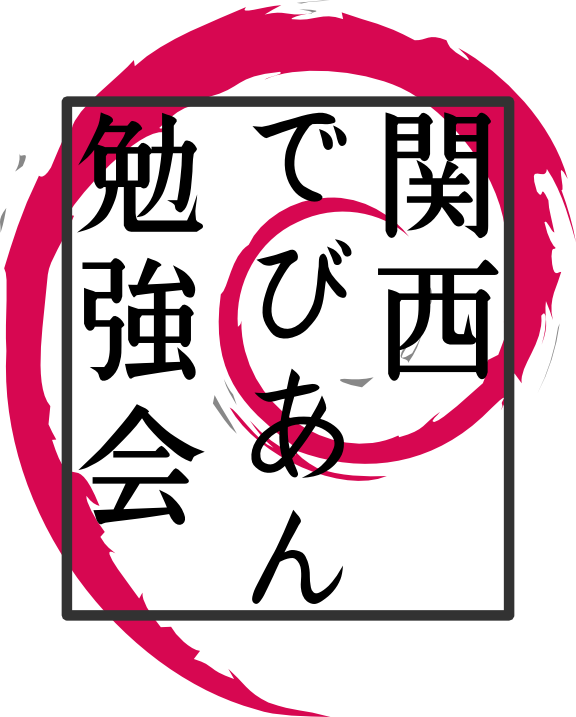
\includegraphics{image200802/kansaidebianlogo.png}
\end{center}

\begin{flushright}
\hfill{}関西 Debian 勉強会担当者 山下 尊也\\
\hfill{}\debmtgyear{}年\debmtgmonth{}月\debmtgdate{}日
\end{flushright}

\thispagestyle{empty}
\end{titlepage}

\dancersection{Introduction}{山下 尊也}
 
 関西 Debian 勉強会はDebian GNU/Linux のさまざ
 まなトピック(新しいパッケージ、Debian 特有の機能の仕組、Debian 界隈で起
 こった出来事、などなど)について話し合う会です。

 目的として次の三つを考えています。
 \begin{itemize}
  \item MLや掲示板ではなく、直接顔を合わせる事での情報交換の促進
  \item 定期的に集まれる場所
  \item 資料の作成
 \end{itemize}

 それでは、楽しい一時をお楽しみ下さい。

\newpage

\begin{minipage}[b]{0.2\hsize}
 {\rotatebox{90}{\fontsize{80}{80}
{\gt 関西デビアン勉強会}}}
\end{minipage}
\begin{minipage}[b]{0.8\hsize}
\hrule
\vspace{2mm}
\hrule
\setcounter{tocdepth}{1}
\tableofcontents
\vspace{2mm}
\hrule
\end{minipage}

\dancersection{最近のDebian関係のイベント報告}{山下 尊也}
\subsection{第10回 関西 Debian 勉強会}
2008年2月23日に「第10回 関西 Debian 勉強会」を行いました。
KURASHIKI Satoruさん、
榎 真治さん、
ujihisaさん、
川江さん、
義田 博一さん、
杉本 典充さん、
大浦 真さん、
甲斐正三さん、
中尾 昌広さん、
川口 美邦さん、
永田昭雄さん、
山嵜 魏さん、
Tatsuya Kinoshitaさん、
名村 知弘さん、
山本高久さん、
ヤマザキ シンイチさん、
岩本 淳二さん、
のがたじゅんさん、
よしだあつしさん、
藤沢理聡さん、
後藤 直久さん、
久保 博さん、
清野 陽一さん、
松嶋 達哉さん、
そして、たかやの合計25名の参加でした。

また、内容は、研究などで Debian を使っている方が、
自分の分野での Debian の使用について講師をして頂きました。

\begin{itemize}
 \item DebianでPCクラスタを作ってみよう 中尾 昌広さん
 \item GIS on Debian GNU/Linux! 清野 陽一さん
 \item 資料作成基礎(TeX) たかや
\end{itemize}

\subsection{OSC 2008 Spring}

2008年2月29日と3月1日の両日に渡って東京新宿で開かれた
「Open Source Conference 2008 Tokyo/Spring」
に東京エリアDebian勉強会有志が参加したため、
お手伝いに行ってきました。
なお、関係者のスケジュールの都合上、
東京エリアDebian勉強会は3月1日のみの参加でした。

関西 Debian 勉強会のメンバーは、
清野さんは午後から用事があったため、午前中のみの
参加で、私、たかやは、午前、午後お手伝いしました。

内容は、やまねさんのセッションは、40人教室に36人と盛況でした。
岩松さんのハンズオンは、初の試みだったので、
課題がいろいろ残ったようです。

\begin{itemize}
 \item Debian Package ハンズオン 岩松 信洋
 \item Debian Overview やまねひでき
\end{itemize}

\newpage

資料は、第37回東京エリアDebian勉強会、2008年 OSC春出張
\footnote{\url{http://tokyodebian.alioth.debian.org/2008-02.html}}
と、やまねさんの資料はスラッシュドットでも
話題\footnote{\url{http://slashdot.jp/linux/08/03/18/0855234.shtml}}になり、
Debian Overview(やまねひでき)
\footnote{\url{http://www.mithril-linux.org/~henrich/debian/osc2008spring.pdf}}
にあります。

\subsection{OSC 2008 Kansai kick-off meeting}
2008年3月11日に京都コンピュータ学院京都駅前校で行われた
OSC 2008 Kansai kick-off meetingに行ってきました。
このミーティングは、昨年のことを踏まえた上で、
今年で2回目となるKyotoでのOSC 2008 Kansaiの方向性について
話合いました。

関西 Debian 勉強会からは、中尾 昌広さん、清野 陽一さん、榎 真治さん、
そして、たかやの合計4人が参加しました。

このミーティングで決まった事は、以下の通りです。

\begin{itemize}
 \item 準備は木曜日から出来る
 \item セッションは去年と同じ
 \item ブースには2から3人がつく(多すぎず、少なすぎず)
 \item 机を壁にくっつける形にし、細かい話などは、
場所を変えて行なうように考慮する(OSC 2008 Springのかたち)
 \item 細かい話などが出来る部屋を用意
 \item rubyやDebianは人が集まるので、角などを提供
 \item ネットワーク環境は前と同じ
 \item ハンズオンは、要望は出せる\\
→VMWareなどの環境か、1CD Linuxを用意する
\end{itemize}

OSCの運用に関することについては、osc-member 案内ページ
\footnote{\url{http://list.ospn.jp/mailman/listinfo/osc-member}}
からメーリングリストに入会して下さい。

また、関西 Debian 勉強会としてイベントに参加したい方は、
イベント専用のメーリングリストがありますので、
私までご連絡下さい。

%%% 木下さん
\dancersection{バグレポートから参加するDebianパッケージ開発}{木下 達也}
\subsection{Debian開発への参加}
Debianは、どんな用途に使ってもよい、ソースを変更できる、
そのままでも変更版でもコピーして配布できる、
自由(フリー)なソフトウェアであり続ける、
ユーザーの、フリーソフトウェアコミュニティのための
オペレーティングシステムです。

Debian Projectは有志によって構成されています。
皆さんのできる範囲での参加・手助けを歓迎します。
まずはバグレポートから……

\begin{itemize}
 \item Debianプロジェクトホームページ \\
       \url{http://www.debian.org/}
 \item Debian社会契約 / Debianフリーソフトウェアガイドライン(DFSG)\\
       \url{http://www.debian.org/social_contract}
 \item How You Can Join\\
       \url{http://www.debian.org/devel/join/}
 \end{itemize}

\subsection{Debianパッケージを使っていて問題に遭遇!}
バグ?
設定誤り?
その他、環境依存の問題など?

さて、どうする?

\subsection{問題解決へ}

\begin{itemize}
 \item 現状は? 望ましい姿は? 再現できる?
 \item 問題の切り分け、仮説、実行、検証
 \begin{itemize}
  \item 設定をデフォルト値(または最小の設定)にしてみると?
  \item その他、条件を変えてみると?
 \end{itemize}
 \item ソースを見てみる?
\begin{commandline}
# apt-get update
(/etc/apt/sources.listにdeb-src行が必要)
$ apt-get source パッケージ名
\end{commandline}
\end{itemize}

\subsection{パッケージ情報の調べ方}

\begin{itemize}
 \item ファイルがどのパッケージに含まれているか検索
       \begin{itemize}
	\item インストール済のパッケージから検索
\begin{commandline}
$ dpkg -S /bin/ls
$ dpkg -S bin/apt
\end{commandline}
 \item Debian Packagesページで「パッケージの内容」を検索\\
 \url{http://packages.debian.org/}
 \item apt-file
\begin{commandline}
# apt-file update
$ apt-file -F search bin/ls
  (キーワードを末尾に持つパス)
$ apt-file search bin/apt
  (キーワードを含む名前のファイルを含むパッケージ)
\end{commandline}
\end{itemize}

\item Debian Bug Tracking System (BTS)\\
バグレポートを記録・追跡\\
\url{http://bugs.debian.org/}\\
\verb|http://bugs.debian.org/パッケージ名|\\
\verb|http://bugs.debian.org/src:ソースパッケージ名|
\end{itemize}

\subsection{メーリングリスト}
\begin{itemize}
\item Debian Mailing Lists\\
\url{http://lists.debian.org/}\\
(バグレポートやアップデート情報はメーリングリストにも流れています)

\item 日本語で相談するには、Debian JP Projectのメーリングリスト\\
\url{http://www.debian.or.jp/community/ml/}\\
\url{http://www.debian.or.jp/community/ml/openml.html}

\item 検索
 \begin{itemize}
 \item Google グループ: \url{http://groups.google.com/}
 \item Gmane Search: \url{http://search.gmane.org/} (日本語検索は難有り)
 \end{itemize}
\end{itemize}

\subsection{バグレポートの書き方}
\begin{itemize}
\item メールクライアントを起動

\item メール作成
 \begin{itemize}
 \item Text/Plainで
 \item 添付やgpg署名は可
 \end{itemize}

\item 宛先、題目を記入
\begin{commandline}
To: submit@bugs.debian.org
Subject: yaskkserv: funny dictionary order when skkdic-extra is installed
\end{commandline}

\item 本文の1行目からパッケージ名、バージョン、重要度を記入
\begin{commandline}
Package: yaskkserv
Version: 0.3.8-1
Severity: wishlist
\end{commandline}

\item Severity(重要度)
 \begin{itemize}
 \item critical (致命的)
 他のパッケージやシステムに影響する重大なバグ
 \item grave (重大)
 そのパッケージ自体の重大なバグ
 \item serious (深刻)
 ポリシー違反など、リリース品質でないと判断されるバグ
 \item important (重要)
 \item normal (通常)
 \item minor (軽度)
 \item wishlist (要望)
 \end{itemize}

\item 1行空けて、本文を記入、送信\\
(例: \url{http://bugs.debian.org/464812})
\begin{commandline}
Date: Sat, 09 Feb 2008 12:45:58 +0900 (JST)
From: Tatsuya Kinoshita <tats@vega.ocn.ne.jp>
To: submit@bugs.debian.org
Subject: yaskkserv: funny dictionary order when skkdic-extra is installed

Package: yaskkserv
Version: 0.3.8-1
Severity: wishlist
    
When the skkdic-extra package is installed, SKK-JISYO.JIS* in
skkdic-extra seem to be prefered over SKK-JISYO.L* in skkdic.
(e.g. when converting "あし", the default setting of yaskkserv
prefers "跫", "蹇", "蹙", ... over "足")

Please prefer SKK-JISYO.L* over SKK-JISYO.JIS* by default.

Thanks,
--
Tatsuya Kinoshita
\end{commandline}

\item Emacsユーザーなら`M-x debian-bug RET'
 \begin{itemize}
 \item 要debian-elパッケージ
 \item MewやWanderlustをデフォルトのEmacsメールクライアントに設定\\
 (/usr/share/doc/パッケージ名/README.Debianを参照)
 \end{itemize}
\end{itemize}

\subsection{Debian開発者との協同}
\begin{itemize}
\item Debian Package Tracking System (PTS)\\
ソースパッケージ毎のまとまった情報ページ\\
\url{http://packages.qa.debian.org/}ソースパッケージ名\\
(パッケージ名でもOK。ソースパッケージのページへ転送されます)

\item PTS subscribe, unsubscribe
 \begin{itemize}
 \item バグレポート、アップロード情報などを購読できる
 \item どの情報を購読するかは、メールでpts@qa.debian.orgへコマンドを送って変更\\
 \url{http://www.debian.org/doc/manuals/developers-reference/ch-resources.en.html}
 \end{itemize}

\item メールアドレス
 \begin{itemize}
 \item バグレポートへの返信: バグ番号@bugs.debian.org
 \item バグレポートの制御: control@bugs.debian.org
 \item パッケージメンテナ宛: パッケージ名@packages.debian.org
 \item Debian開発者宛、セキュリティ情報、非公開: security@debian.org
 \item Debianセキュリティチーム宛、非公開: team@security.debian.org
 \end{itemize}
\end{itemize}

%%% 倉敷さん
\dancersection{GPG 最初の一歩}{倉敷 悟}

GnuPG というと、「ああ、なんか apt-get の時にゴチャゴチャ文句言ってくる
アレか」といった印象をお持ちの方もおられるのではないかと思います。実は
Debian には様々な形で GPG が組みこまれていて、ssh 等にならぶマスト
アイテムといっても過言ではありません。このセッションでは、GPG の用途と
役割について簡単にご紹介した後、典型的な使用方法についてデモを行います。

\subsection{GPG の概要}

端的に GPG とは何か、というと:
\begin{itemize}
 \item PGP 規格のフリーな実装 (特許の観点で、あるいは処理系として)
       \begin{itemize}
        \item 公開鍵暗号と共通鍵暗号のハイブリッド方式
       \end{itemize}
 \item メールやファイルの暗号化をするソフト
       \begin{itemize}
        \item 暗号化で盗聴を防ぐ (機密性/Confidentiality)
        \item 署名で改竄を防ぐ (完全性/Integrity)
        \item 信頼の輪で本人同定 (認証/Authentication)
       \end{itemize}
\end{itemize}

より詳しい解説は、下記 URL で読むことができます。

\begin{itemize}
 \item The GNU Privacy Guard \url{http://gnupg.org/} \\
       GnuPG 本家。ドキュメントは豊富ですが全部英語です。
 \item GNU Privacy Guard 講座 \url{http://hp.vector.co.jp/authors/VA019487/} \\
       日本語のポータル的なサイト。使い方を調べたい時に最適かと思います。       
 \item GnuPG (The GNU Privacy Guard) \url{http://www.math.s.chiba-u.ac.jp/~matsu/gpg/index.html} \\
       少し古い記事ですが、暗号機能の一般的な背景がわかりやすく解説されています。
\end{itemize}

\subsection{Debian における GPG}


\subsubsection{パッケージアーカイブ}

etch 以降、配布しているパッケージアーカイブの改竄防止のため、Release
ファイルに GPG でデジタル署名を施しています。APT でパッケージを取得する
際に、この署名を確認して、検証できない場合は警告が表示されるようになっています。

公式アーカイブの公開鍵はパッケージとして配布されているので、これをインス
トールしておけば、後は APT がよしなに面倒をみてくれます。

\begin{commandline}
kura@acacia:~$ dpkg -l | grep keyring
ii  debian-archive-keyring               2007.07.31                    GnuPG archive keys of the Debian archive
ii  debian-multimedia-keyring            2007.02.14                    GnuPG archive key of the debian-multimedia r
\end{commandline}

上記の例では debian-multimedia の鍵も入っていますが、公式でない
アーカイブでも、鍵が配布されていれば同じように検証をしてくれます。

\begin{itemize}
 \item SecureApt \url{http://wiki.debian.org/SecureApt}
\end{itemize}

\subsubsection{開発者の認証}

Debian では、GnuPG が本人の身分証明手段として広く浸透しており、特に
パッケージまわりで作業しようと思うと、なんだかんだで必要になります。

私に見えてる範囲では:
\begin{itemize}
 \item keysign に必要 (本末転倒ですが……)
 \item パッケージのビルドに必要 (必須ではない)
 \item mentors.debian.net への登録に必要
 \item Debian JP への参加に必要
 \item Debian {Maintainer|Developer} への応募に必要
\end{itemize}
といった場面で自分の GPG 鍵が必要です。また、ただ作るだけではなくて、
Debian Developer と keysign を行っておく必要もあります。

\subsection{名刺としての GPG 鍵}

現時点では、「Debian は使うだけだし、面倒だから別に要らないや」と
思うかも知れません。

ただ、他にもメリットがありますし、これを機会に是非 GnuPG を
使ってみてください。最初に必要なのは、たった一つ、「これから
作る鍵をちゃんと維持するぞ」という意気込みだけです。

\begin{itemize}
 \item デジタルな identity として
 \item こういったコミュニティでの名刺交換に
 \item 公開鍵基盤の身近な活用例として
 \item Debian Developer はレア
 \item keysign は結構おもしろい
\end{itemize}

\subsection{はじめてみよう}

\subsubsection{GPG 鍵を作る}
というわけで、自分の鍵を作ってみましょう。

\begin{commandline}
kura@acacia:~$ gpg --gen-key
gpg (GnuPG) 1.4.6; Copyright (C) 2006 Free Software Foundation, Inc.
This program comes with ABSOLUTELY NO WARRANTY.
This is free software, and you are welcome to redistribute it
under certain conditions. See the file COPYING for details.

gpg: directory `/home/kura/.gnupg' created
gpg: can't open `/gnupg/options.skel': そのようなファイルやディレクトリはありません
gpg: keyring `/home/kura/.gnupg/secring.gpg' created
gpg: keyring `/home/kura/.gnupg/pubring.gpg' created
Please select what kind of key you want:
   (1) DSA and Elgamal (default)
   (2) DSA (sign only)
   (5) RSA (sign only)
Your selection? 
\end{commandline}

まず、鍵の種類を聞かれます。ここはデフォルトのままで構いませんので、
何も入力せずに enter を押します。

\begin{commandline}
DSA keypair will have 1024 bits.
ELG-E keys may be between 1024 and 4096 bits long.
What keysize do you want? (2048) 
\end{commandline}

次に、鍵の流さを聞かれます。選択の目安としては、1024 は短かすぎるので NG、
デフォルトの 2048 はまぁ OK、計算機資源が余っているなら 4096 もアリ、
といったところでしょうか。

この例では、そのまま enter を押して、デフォルトの 2048 としています。

\begin{commandline}
Requested keysize is 2048 bits
Please specify how long the key should be valid.
         0 = key does not expire
      <n>  = key expires in n days
      <n>w = key expires in n weeks
      <n>m = key expires in n months
      <n>y = key expires in n years
Key is valid for? (0) 
Key does not expire at all
Is this correct? (y/N) y
\end{commandline}

次は、鍵の有効期限を選びます。私の場合、最初ここをどうするべきか困ったと
ころですが、これまで keysign してもらった方々のを見る限り、期限なしで問題
ないようです。

というわけで、そのまま enter を押して、確認にも y と答えます。

\begin{commandline}
You need a user ID to identify your key; the software constructs the user ID
from the Real Name, Comment and Email Address in this form:
    "Heinrich Heine (Der Dichter) <heinrichh@duesseldorf.de>"

Real name: KURASHIKI Satoru
Email address: lurdan@gmail.com
Comment: 
\end{commandline}

ここでは、自分の個人情報を設定します。keysign などでは、公的な証明書との
つきあわせを行いますので、その時に確認できる本名を入力する必要があります。
このあたり、日本のネットワーク文化とはいまひとつ馴染みがよくないかも知れ
ませんね。

GPG 鍵では、一つの ID に対して複数のメールアドレスを設定することができる
ので、Comment でそれを明示することができます。

\begin{commandline}
You selected this USER-ID:
    "KURASHIKI Satoru <lurdan@gmail.com>"

Change (N)ame, (C)omment, (E)mail or (O)kay/(Q)uit? O
\end{commandline}

最終的に、ユーザ ID がこうなりますよ、という確認です。問題ないので
O と入力します。

\begin{commandline}
You need a Passphrase to protect your secret key.

Enter passphrase:
Repeat passphrase: 
\end{commandline}

ここでパスフレーズを確認含めて 2 回入力します。パスフレーズには流さの
制限がないので、覚えやすい長さの英文を使うといいのではないでしょうか。

\begin{commandline}
We need to generate a lot of random bytes. It is a good idea to perform
some other action (type on the keyboard, move the mouse, utilize the
disks) during the prime generation; this gives the random number
generator a better chance to gain enough entropy.
.+++++++++++++++..++++++++++.++++++++++++++++++++++++++++++++++++++++.+++++++++++++++.+++++++++++++++.+++++.++
++++++++++++++++++.++++++++++>.++++++++++..............+++++

Not enough random bytes available.  Please do some other work to give
the OS a chance to collect more entropy! (Need 230 more bytes)
We need to generate a lot of random bytes. It is a good idea to perform
some other action (type on the keyboard, move the mouse, utilize the
disks) during the prime generation; this gives the random number
generator a better chance to gain enough entropy.
++++++++++......+++++..+++++.+++++.+++++.+++++..++++++++++.+++++.+++++++++++++++..+++++.++++++++++....+++++.++
+++++++++++++.++++++++++.++++++++++.+++++..+++++++++++++++..+++++>.++++++++++...>.+++++.......................
..............................................................................................................
...............+++++^^^^^
\end{commandline}

パスフレーズを入力した後は、乱数の生成のために、ブラウザでも開いて適当
に別の作業をします。そろそろいいかな、と元の画面に戻ると……

\begin{commandline}
gpg: /home/kura/.gnupg/trustdb.gpg: trustdb created
gpg: key 9751B54D marked as ultimately trusted
public and secret key created and signed.

gpg: checking the trustdb
gpg: 3 marginal(s) needed, 1 complete(s) needed, PGP trust model
gpg: depth: 0  valid:   1  signed:   0  trust: 0-, 0q, 0n, 0m, 0f, 1u
pub   1024D/9751B54D 2008-03-21
      Key fingerprint = 3AAA 2ED1 ACDA 49AE 4C68  66B9 CE7D E89C 9751 B54D
uid                  KURASHIKI Satoru <lurdan@gmail.com>
sub   2048g/B79D76D0 2008-03-21
\end{commandline}

このように完成しています。最後に表示された 「key fingerprint」のうち、
最後の 2 ブロックが自分の鍵の ID となります。

最後に表示されている部分で、「pub」の行が公開鍵、「sub」の行が秘密鍵を表
しています。

\begin{commandline}
kura@acacia:~$ ls -l .gnupg
合計 20
-rw------- 1 kura kura 1167 2008-03-21 16:06 pubring.gpg
-rw------- 1 kura kura 1167 2008-03-21 16:06 pubring.gpg~
-rw------- 1 kura kura  600 2008-03-21 16:06 random_seed
-rw------- 1 kura kura 1316 2008-03-21 16:06 secring.gpg
-rw------- 1 kura kura 1280 2008-03-21 16:06 trustdb.gpg
\end{commandline}

生成された鍵は、このように \$HOME/.gnupg/ に保管されています。これらの
ファイルは超大事なので、大切に取り扱うようにしましょう。

ちなみに、上の例で使っている鍵は、この記事のために作ったもので、もはや
存在しません。

\subsubsection{基本的な操作}

通常は、自分の鍵束 (\$HOME/.gnupg/*) には、

\begin{itemize}
 \item 自分の秘密鍵
 \item 自分の公開鍵
 \item 他の人の公開鍵
\end{itemize}

が入っています。これらの情報を確認する基本的なコマンドをご紹介します。
なお、鍵束の中で特定の鍵を指定するには、次のうちどれかが使えます。

\begin{itemize}
 \item 鍵 ID (ex. 0x9751B54D)
 \item 鍵 ID の 0x を省略 (ex. 9751B54D)
 \item 自分の UID の一部 (ex. KURA)
\end{itemize}
       
自分の鍵束にある公開鍵を一覧表示:
\begin{commandline}
$ gpg --list-keys
\end{commandline}

そのうち特定の公開鍵を表示:
\begin{commandline}
$ gpg --list-keys KURA
\end{commandline}

鍵指紋 (fingerprint) を確認:
\begin{commandline}
$ gpg --fingerprint KURA
\end{commandline}

鍵署名を確認:
\begin{commandline}
$ gpg --list-sigs KURA
\end{commandline}

\subsubsection{メールで使ってみる}

私が GPG を使うのは、主に gmail 上のメールアドレスなので、firefox のプラ
グイン「firegpg」を使っています。対象となる本文を選択して増えたボタンを
押すだけなので簡単に使うことができます。

\subsection{keysign の流れ}

\subsubsection{準備}

keysign のためには、次のものが必要です。

\begin{itemize}
 \item 公的な証明書 (鍵の持ち主の個人情報を証明できる、写真つきの書類)
       \begin{itemize}
        \item 運転免許
        \item 住民基本台帳カード
        \item パスポート
        \item 学生証
       \end{itemize}
 \item 署名してもらう鍵の指紋 (fingerprint) を印刷したもの
\end{itemize}

私の場合、鍵の指紋は手で書いたり、鍵表示をそのままコピペして印刷したり
していました。

\begin{commandline}
pub   1024D/9751B54D 2008-03-21
      Key fingerprint = 3AAA 2ED1 ACDA 49AE 4C68  66B9 CE7D E89C 9751 B54D
uid                  KURASHIKI Satoru <lurdan@gmail.com>
sub   2048g/B79D76D0 2008-03-21
\end{commandline}

\subsubsection{当日}

公的な証明書を使って、keysign の相手とお互いに相手が相手であること
を確認し、用意した鍵指紋 (fingerprint) の印刷を交換します。

これだけです。簡単ですね。

\subsubsection{その後}

端末の前に戻ったら、まずは相手の公開鍵を手に入れましょう。

\begin{commandline}
$ gpg --keyserver subkeys.pgp.net --recv-keys 0x????????
\end{commandline}

keyserver は、相手が Debian Developer であれば keyring.debian.org も使え
ます。また、? の部分には、もらった鍵指紋 (fingerprint) の最後の 8 文字を入力します。

無事に公開鍵が入手できたら、それに署名をします。

\begin{commandline}
$ gpg --edit-key 0x????????
\end{commandline}

gpg のコマンドモードに入るので、
「uid (数字)」で署名をする uid を選び
(*マークがつきます)、
「sign」と入力します(fingerprint とメールアドレスを確認して署名)。

なお、相手が複数の uid を持っている場合、私は一通り全てに署名することに
しています。

終わったら、「quit」と入力し、変更を保存してください。

次のように署名の結果を表示して、自分の名前が表示されていることを確認してください。

\begin{commandline}
$ gpg --list-sigs 0x????????
\end{commandline}

ここまでで問題がなければ、相手の公開鍵をテキストファイルに export します。

\begin{commandline}
$ gpg --export -a  0x???????? > someones.key
\end{commandline}

後は、これを相手に送るだけです。添付するなり、本文に貼るなりして、メール
で送信します。相手の公開鍵で暗号化しておくとよいでしょう。

さて、相手も同じように署名をしてくれているはずですので、しばらくすると
メールで自分の公開鍵を送ってもらえるはずです。

届いたら、テキストファイルに export された鍵を自分の鍵束にとりこみ、
ついでなので公開鍵サーバにも送っておきます。
\begin{commandline}
$ gpg --import yours.key
$ gpg --keyserver subkeys.debian.org --send-keys 0x????????
\end{commandline}

? には、自分の公開鍵 ID を入力します。

\begin{itemize}
 \item 鍵署名 (Keysigning) \url{http://www.debian.org/events/keysigning}
\end{itemize}

%%% 大浦さん
\dancersection{Debian 開発者のコーナーの歩き方}{大浦 真}

Debian プロジェクトの Web ページ内の
「Debian 開発者のコーナー」(\url{http://www.debian.org/devel/}) には、
Debian の開発や改良を行っていくために必要な情報が集まっている。
ただ、いろいろあり過ぎて、どこに何があるか分かりにくい。
以下、有用なものをいくつか紹介する。

\subsection{基本}

プロジェクトに関する基本的な情報。
\begin{itemize}
\item Debian の組織構成
\item Debian に参加する
\item 開発者データベース --- Debian 開発者の情報やプロジェクトのマシンを
  検索できる。
\item 投票情報 --- 現在 2008年度プロジェクトリーダの選挙期間中。
\item さまざまなアーキテクチャ --- Debian は i386 以外にも多くのアーキテクチャに
  移植されている。
  Linux 以外への移植もある。
\end{itemize}

\subsection{パッケージ開発}

パッケージを作成、メンテナンスするために必要な情報。
メンテナが読むべき文書が集まっている。

\begin{itemize}
\item Debian ポリシーマニュアル --- Debian のシステムが守るべき技術的事項。
  いくつかサブポリシーもある。
\item デベロッパーズリファレンス --- Debian のメンテナが守るべき手順と
  利用できるリソースの情報。
\item 新規メンテナのためのガイド
\end{itemize}

\subsection{進行中の仕事}

パッケージのメンテナンスを進めていくために必要な情報。

\begin{itemize}
\item バグ追跡システム
\item パッケージ追跡システム
\item Lintian レポート --- パッケージがポリシーを満たしているかどうか
  チェックする。
\end{itemize}

\subsection{プロジェクト}

Debian 内のプロジェクトに関するリンク。

\begin{itemize}
\item 品質保証 (Quality Assurance) グループ --- Debian 全体の品質を
  向上させるためのプロジェクト
\item 自動構築ネットワーク --- ソースパッケージを各アーキテクチャ用に
  自動的に構築する。
\item いろいろなカスタム Debian ディストリビューション
\end{itemize}

\subsection{その他}

その他の情報。

\begin{itemize}
\item Debian の ロゴとバナー
\end{itemize}

\dancersection{今後の予定}{山下 尊也}

\subsection{次回}
次回は、2008年04月29日に姫路獨協大学駅前サテライト
\footnote{\url{http://www.himeji-du.ac.jp/satellite/index.html}}
にて行なう予定です。

また、ネット環境があるので、
USTREAM.TV\footnote{\url{http://www.ustream.tv/}}にて、
ビデオカンファレンスを開こうと考えています。

\subsection{OSC 2008 Kansaiについて}
今年のOSC Kansaiの日程が決まりました。
7月18,19日(金・土)に行なわれます。

関西 Debian 勉強会として決まっているのは、
以下の通りです。

\begin{itemize}
 \item 18日に参加出来る方が多ければ、18日,19日両日参加する
 \item セッション時間は、2時間頂き、通常とほぼ同様の勉強会を開催する
 \item ブース担当と、セッション担当に分ける
\end{itemize}

\subsection{KDRのおしらせ}
関西Debian勉強会の有志で
関西Debian勉強会とは独立した形で、
週に一度、読書会(KDR)を開いています。
詳しくはKDR公開用ページ\footnote{\url{http://qwik.jp/kdrweb/}}をご覧下さ
い。

\dancersection{メモ}{}

\mbox{}\newpage
 
\printindex
 \cleartooddpage

 \begin{minipage}[b]{0.2\hsize}
  \rotatebox{90}{\fontsize{80}{80} {\gt 関西デビアン勉強会} }
 \end{minipage}
 \begin{minipage}[b]{0.8\hsize}

 \vspace*{15cm}
 \rule{\hsize}{1mm}
 \vspace{2mm}
 
\includegraphics[width=2cm]{image200502/openlogo-nd.eps}
 \noindent \Large \bf Debian 勉強会資料\\ \\
 \noindent \normalfont \debmtgyear{}年\debmtgmonth{}月\debmtgdate{}日 \hspace{5mm}  初版第1刷発行\\
 \noindent \normalfont 関西 Debian 勉強会 (編集・印刷・発行)\\
 \rule{\hsize}{1mm}
 \end{minipage}

\end{document}
